% !TeX root = RJwrapper.tex
\title{exvatools: Value Added in Exports and Other Input-Output Table Analysis Tools}
\author{by Enrique Feás}

\maketitle

\abstract{%
This article introduces an R package, \CRANpkg{exvatools}, that simplifies the analysis of trade in value added with international input-output tables. It provides a full set of commands for data extraction, matrix creation and manipulation, decomposition of value added in gross exports (using alternative methodologies) and a straightforward calculation of many value added indicators. It can handle both raw data from well-known public input-output databases and custom data. It has a wide sector and geographical flexibility and can be easily expanded and adapted to specific economic analysis needs, facilitating a better understanding and a wider use of the available statistical resources to study globalization.
}

\hypertarget{introduction}{%
\section{Introduction}\label{introduction}}

The analysis of trade in value added involves the use of international
input-output tables and intensive matrix manipulation. Some trade databases,
such as the OECD Trade in Value Added Database (TiVA), offer a web interface,
but cannot be customized and lack some key indicators developed in recent
literature, especially indicators of bilateral trade in value added and
participation in global value chains. This makes recourse to raw data almost
inevitable and creates the need for software capable of performing complex
matrix analysis in a user-friendly environment.

This is the gap \CRANpkg{exvatools} pretends to fill. It has been designed as a
package for \textbf{R} with a triple purpose: as an international input-output table
general analysis tool (with commands to extract raw data and produce and
manipulate large matrices), as a way to decompose value added in exports using
alternative methodologies, and as a tool to easily produce complex tailor-made
value added indicators with flexible sector and geographical customization.

To our knowledge, there are no equivalent software tools available. There are
some input-out analysis tools, like \CRANpkg{ioanalysis}
(Wade and Sarmiento-Barbieri 2020), but they cannot properly handle OECD's ICIO-type data
(with some countries divided in industrial areas). The package \CRANpkg{decompr}
(Quast and Kummritz 2015) produces a decomposition of value added in exports, but
only according to the methodology of Wang, Wei, and Zhu (2013).

Outside of the \textbf{R} ecosystem, the module \texttt{icio} (Belotti, Borin, and Mancini 2021) for the
software \textbf{Stata} (StataCorp 2021) provides the more modern (and
methodologically sounder) decomposition method of Borin and Mancini (2023).
However, \texttt{icio} is a closed-source module, it does not allow complex sector
analysis and customization, direct handling of input-output tables nor detailed
decompositions (for instance, distinguishing between value added exported
induced by inputs and by final goods).

\CRANpkg{exvatools} can therefore be used as all-purpose tool, both to
facilitate the extraction and manipulation of input-output matrices and to
obtain detailed and customized indicators of trade in value added, facilitating
research on global value chains, globalization, and its economic effects. In the
following sections, we will describe the methodological background of
\CRANpkg{exvatools}, in particular the international input-output table
framework and its use to calculate value added induced by gross exports. Then we
will explain the creation of the three basic objects of \CRANpkg{exvatools}: a
list of basic input-output tables (the \texttt{wio} class), a list with the different
matrix components of a decomposition of value added in exports (the \texttt{exvadec}
class) and a list with a detailed origin and destination of value added (the
\texttt{exvadir} class). We will then explain the commands to fully exploit the
information included in the aforementioned classes. Along the way we will
produce examples of use.

\CRANpkg{exvatools} can be installed from the CRAN repository and made
available for the current session following the usual procedure:

\begin{verbatim}
install.packages("exvatools")
library(exvatools)
\end{verbatim}

\hypertarget{background-methodology}{%
\section{Background methodology}\label{background-methodology}}

\hypertarget{the-international-input-output-framework}{%
\subsection{The international input-output framework}\label{the-international-input-output-framework}}

Analyzing the value added in exports requires the previous extraction of a
series of basic input-output matrices in a standardized format. We will consider
a typical international input-output framework with \(G\) countries and \(N\)
sectors. Each country \(s\) provides goods and services from each sector \(i\) to
each sector \(j\) in country \(r\), and sources its goods and services from the
sectors of each country \(t\).

\begin{table}[h]
    \centering
    \caption{\label{tab:iot}Structure of an international Input-Output Table}
    \begin{tabular}{|lc|c|c|c|c|c|c|c|c|c|}
        \hline
        \multicolumn{2}{|r|}{Output}
        & \multicolumn{4}{|c|}{Intermediate uses}
        & \multicolumn{4}{|c|}{Final uses}
        & Output \\ \cline{3-10}
        \multicolumn{2}{|l|}{Input} & 1 & 2 & ... & $G$
        & 1 & 2 & ... & $G$ & ~ \\ \hline
        ~ & 1 & $\mathbf{Z}_{11}$ & $\mathbf{Z}_{12}$ & ... & $\mathbf{Z}_{1G}$ &
        $\mathbf{Y}_{11}$ & $\mathbf{Y}_{12}$ & ... & $\mathbf{Y}_{1G}$
        & $\mathbf{X}_{1}$ \\
        Intermediate & 2 &
        $\mathbf{Z}_{21}$ & $\mathbf{Z}_{22}$ & ... & $\mathbf{Z}_{2G}$ &
        $\mathbf{Y}_{21}$ & $\mathbf{Y}_{22}$ & ... & $\mathbf{Y}_{2G}$ &
        $\mathbf{X}_{2}$ \\
        inputs & ... & ... & ... & ... & ... & ... & ... & ... & ... & ... \\
        ~ & $G$ & $\mathbf{Z}_{G1}$ & $\mathbf{Z}_{G2}$ & ... & $\mathbf{Z}_{GG}$
        & $\mathbf{Y}_{G1}$ & $\mathbf{Y}_{G2}$ & ... & $\mathbf{Y}_{GG}$ &
        $\mathbf{X}_{G}$ \\ \hline
        Value added & ~ & $\mathbf{VA}_{1}$ & $\mathbf{VA}_{2}$ & ... &
        $\mathbf{VA}_{G}$ \\ \cline{1-6}
        Input & ~ & $\mathbf{X}_{1}$ & $\mathbf{X}_{2}$ & ...
        & $\mathbf{X}_{G}$  \\ \cline{1-6}
    \end{tabular}
\end{table}

In a typical international input-output table (which is a matrix composed of
block matrices) \(\mathbf{Z}\) is the matrix of intermediate inputs (dimension \(GN \times GN\)), with each sub-matrix \(\mathbf{Z}_{sr}\) (dimension \(N \times N\))
elements \(z_{sr}^{ij}\) representing the deliveries of intermediate inputs from
sector \(i\) in country \(s\) to sector \(j\) in country \(r\). \(\mathbf{Y}\) is the
matrix of final demand, of dimension \(GN \times G\) (aggregated by country for
practical purposes from an original \(\mathbf{Yfd}\) matrix with \(FD\) demand
components). \(\mathbf{X}\) is the production matrix, of dimension \(GN \times 1\),
and \(\mathbf{VA}\) the value added demand, of dimension \(1 \times GN\).

\hypertarget{the-demand-model}{%
\subsection{The demand model}\label{the-demand-model}}

The typical demand model, which dates back to
Leontief (1936), assumes that the inputs from sector \(i\) of country
\(s\) to sector \(j\) of country \(r\) are a constant proportion of the output of
sector \(j\) in country \(r\). From there we obtain a matrix of coefficients
\(\mathbf{A}\) whose elements are the proportion of intermediate inputs over total
production, \(a_{sr}^{ij} = z_{sr}^{ij} / {x_{r}^{j}}\). Then the relations in the
international input-output table can be expressed as
\(\mathbf{AX}+\mathbf{Y}=\mathbf{X}\), from where we deduct a relation between
production and final demand:

\begin{equation}
  \mathbf{X}=\left(\mathbf{I}-\mathbf{A}\right)^{-1}\mathbf{Y}=\mathbf{BY}
   \label{eq:XBY}
\end{equation}

Here the matrix \(\mathbf{B}\) (inverse of \(\mathbf{I} -\mathbf{A}\), where
\(\mathbf{I}\) is the identity matrix) collects the backward linkages that the
final demand \(\mathbf{Y}\) induces on production. Each element of \(\mathbf{B}\),
\(b_{sr}^{ij}\), can be expressed as the increase of production of sector \(i\) in
country \(s\), when the final demand of sector \(j\) in country \(r\) increases by one
unit.

\hypertarget{value-added-in-trade}{%
\subsection{Value added in trade}\label{value-added-in-trade}}

If the ratio between inputs and production is constant, then the ratio between
value added (i.e., the value of production minus the value of inputs) and
production can also be considered constant, so we can define vector \(\mathbf{V}\)
as the value added by unit of output \(\mathbf{X}\) and express the value added in
terms of global demand as \(\mathbf{V} \mathbf{X} = \mathbf{V} \mathbf{BY}\). More
specifically, for a given country \(s\):

\begin{equation}
  \mathbf{V}_s \mathbf{X}_s =
    \mathbf{V}_s \sum_{j}^{G}\sum_{r}^{G}{\mathbf{B}_{sj} \mathbf{Y}_{jr}}
    \label{eq:VBY}
\end{equation}

that we can break down into the value added produced and absorbed in \(s\) and the
value added produced in \(s\) and absorbed abroad:

\begin{equation}
  \mathbf{V}_s \sum_{j}^{G}{\mathbf{B}_{sj}\mathbf{Y}_{js}} +
    \mathbf{V}_s \sum_{j}^{G} \sum_{r\neq s}^{G} {\mathbf{B}_{sj}\mathbf{Y}_{jr}}
    \label{eq:VADVAX}
\end{equation}

The second term in \eqref{eq:VADVAX} is usually referred to as value added
exported \({\mathbf{VAX}}_s\) (Johnson and Noguera 2012). In aggregated terms,
value added absorbed abroad coincides with value added exported, but this is not
true in bilateral terms. In fact, \({\mathbf{VAX}}_{sr}\) is the value added
produced in \(s\) and absorbed in \(r\), but \emph{regardless of the export destination}.
To obtain the value added exported to \(r\) \emph{regardless of the absorption country}
we need to calculate the value added induced not by final demand, but by the
demand of gross exports.

For that, knowing that each column of the matrix product
\(\mathbf{V} \mathbf{B}\) is a linear combination whose sum is a unit vector
\(\boldsymbol{\iota}\), we can break down the linkage effects over the production
of any country \(s\) into those derived of domestic inputs and those derived of
foreign components.

\begin{equation}
    \boldsymbol{\iota} = \sum_{t}^{G}{{\mathbf{V}}_t\mathbf{B}_{ts}} =
    {\mathbf{V}}_s \mathbf{B}_{ss} + \sum_{t\neq s}^{G}
    {{\mathbf{V}}_t\mathbf{B}_{ts}}
     \label{eq:sumVB}
\end{equation}

If we multiply both terms of equation \eqref{eq:sumVB} by the demand of gross
exports of country \(s\), \(\mathbf{E}_s\), we obtain a basic decomposition of the
content of value added in exports into domestic and foreign content.

\begin{equation} 
    \boldsymbol{\iota} \mathbf{E}_{s}
    = \sum_{t}^{G} {{\mathbf{V}}_t\mathbf{B}_{ts}\mathbf{E}_{s}}
    = {\mathbf{V}}_s \mathbf{B}_{ss} \mathbf{E}_{s} +
    \sum_{t\neq s}^{G}{{\mathbf{V}}_t \mathbf{B}_{ts} \mathbf{E}_{s}}
    \label{eq:content}
\end{equation}

Expression \eqref{eq:content} reflects that the demand of gross exports of \(s\)
can only be satisfied with domestic value added or with foreign value added
(with inputs being value added of other sectors). This is also valid for the
bilateral exports of \(s\), \(\mathbf{E}_{sr}\) (the sum being in this case the
total gross bilateral exports).

We have so far overlooked the sector distribution of exports. It we wanted to
preserve the sector information, we should use a diagonalized version of matrix
\(\mathbf{V}\), \(\hat{\mathbf{V}}\), with the resulting product \(\hat{\mathbf{V}} \mathbf{B}\) reflecting the sector of origin of value added. If we opted instead
(as it normally the case) to reflect the value-added exporting sector, then the
products \({\hat{\mathbf{V}}}_s \mathbf{B}_{ss}\) and \({\hat{\mathbf{V}}}_t \mathbf{B}_{ts}\) should be diagonalized as \(\widehat{{\mathbf{V}}_s \mathbf{B}_{ss}}\) and \(\widehat{{\mathbf{V}}_t \mathbf{B}_{ts}}\), respectively.

The decomposition of value added in exports essentially consists in
analyzing the elements of Equation \eqref{eq:content}, extracting the elements
that are not really value added (double counted) as well as those that are
not really exports (flows eventually re-imported and absorbed domestically).

\hypertarget{creating-and-manipulating-input-output-matrices}{%
\section{Creating and manipulating input-output matrices}\label{creating-and-manipulating-input-output-matrices}}

\hypertarget{usage}{%
\subsection{Usage}\label{usage}}

The basic matrices of a Leontief demand-induced model can be easily obtained
from raw data with the command \texttt{make\_wio()}:

\begin{verbatim}
make_wio(wiotype = "icio2023", year = NULL, 
         src_dir = NULL, quiet = FALSE)
\end{verbatim}

where:

\begin{itemize}
\tightlist
\item
  \texttt{wiotype} is a string specifying the type of international input-output table
  to be used (and therefore the source zip file to be looked for in the source
  directory \texttt{src\_dir}).
\item
  \texttt{year} is an integer specifying the reference year. If missing, \texttt{make\_wio()}
  will use the last available year for that database (e.g., 2020 for
  \texttt{"icio2023"} or 2014 for \texttt{"wiod2016"}).
\item
  \texttt{src\_dir} is the source directory where the raw data is located. If data is
  stored in the current working directory, this argument can be omitted.
\item
  \texttt{quiet} is a boolean, with \texttt{TRUE} opting for a silent output.
\end{itemize}

\hypertarget{source-data}{%
\subsection{Source data}\label{source-data}}

\CRANpkg{exvatools} produces basic input-output tables from three types
of data: public international input-output databases, custom data and
sample data.

Public international input-output databases can be directly downloaded from the
web pages of their respective institutions. Three sources are currently
supported:

\begin{itemize}
\tightlist
\item
  OECD Inter-Country Input-Output (ICIO) tables (OECD 2023), on which
  the OECD's Trade in Value Added database (TiVA) is based,
\item
  World Input Output Database (WIOD) tables (Timmer et al. 2015).
\item
  FIGARO EU Input-Output Tables (EU IC-SUIOTs) (Remond-Tierrez and Rueda-Cantuche 2019)
\end{itemize}

The default \texttt{wiotype} is \texttt{"icio2023"}, corresponding to the OECD ICIO Tables,
version 2023 (years 1995 to 2020), available as zip files that can be downloaded
from the \href{https://www.oecd.org/sti/ind/inter-country-input-output-tables.htm}{ICIO web
page}. Older
versions of OECD ICIO (\texttt{"icio2021"}, \texttt{"icio2018"} and \texttt{"icio2016"}) are provided
for backward compatibility (for example, to reproduce examples in literature
using those databases). For WIOD Tables, versions included are \texttt{"wiod2016"}
(version 2016, years 2000 to 2014), \texttt{"wiod2013"} and \texttt{"lrwiod2022"} (long-run
WIOD tables, version 2022, for years 1965 to 2000). All of them are available at
the University of Groningen's \href{https://www.rug.nl/ggdc/valuechain/wiod/}{Growth and Development Centre web
page}. FIGARO tables, whether
industry-by-industry (\texttt{"figaro2022i"}) or product-by-product (\texttt{"figaro2022p"})
are available at the \href{https://ec.europa.eu/eurostat/web/esa-supply-use-input-tables/database}{Eurostat web
page}.

The advantage of these databases is threefold: they are widely used in the
economic literature, they are quite rich in terms of countries and sectors, and
they are directly downloadable from the web page of their supporting
institutions, typically as zipped files containing comma-delimited files
(\texttt{.csv}), Excel files (\texttt{.xlsx}) or R data files (\texttt{.RData}). In any case,
\CRANpkg{exvatools} can be easily extended to other available international
input-output databases like the Eora database (Lenzen et al. 2013) or the ADB
Multi-Regional Input Output (ADB-MRIO) Database
(Asian Development Bank 2023).

For instance, if we want to use \CRANpkg{exvatools} with the 2023 edition of the
OECD ICIO tables (with data up to 2020), we must first download the source file
``ICIO\_2016-2020-extended.zip'' (92 MB) from the \href{https://www.oecd.org/sti/ind/inter-country-input-output-tables.htm}{ICIO web
page}. Then
we will use the command \texttt{make\_wio()}, specifying the edition, the year and the
folder where the source zip file is saved (just the directory). For instance, if
the file was located in \texttt{C:\textbackslash{}Users\textbackslash{}Username\textbackslash{}Documents\textbackslash{}R} and we wanted the year
2020:

\begin{verbatim}
wio <- make_wio("icio2023", year = 2020, 
                src_dir = "C:/Users/Username/Documents/R")
\end{verbatim}

and \CRANpkg{exvatools} will take care of the rest: it will extract the
\texttt{.csv} files from the zip file and produce the basic input-output matrices.

Alternatively, \CRANpkg{exvatools} can use custom data to create basic
input-output matrices. In this case, we just need as input a numeric matrix or
data frame with the intermediate inputs \(\mathbf{Z}\) and the final demand
\(\mathbf{Yfd}\), plus a vector with the names of the countries. In this case, we
will use an alternative command, \texttt{make\_custom\_wio()}.

\begin{verbatim}
wio <- make_custom_wio(df, g_names = c("C01", "C02", "C03"))
\end{verbatim}

If we just want to check the features of \CRANpkg{exvatools}, there is no need
to download any data. The package includes two sets of fictitious data,
\texttt{wiotype\ =\ "iciotest"} (an ICIO-type data sample, with Mexico and China
disaggregated) and \texttt{wiotype\ =\ "wiodtest"} (a WIOD-type data sample). Both can
be directly used in \texttt{make\_wio()}, with no need to specify year or source
directory.

As the dimension of publicly available input-output matrices is big,
here we will use here ICIO-type fictitious data made with
\texttt{make\_wio("iciotest")}.

\begin{verbatim}
wio <- make_wio("iciotest")
\end{verbatim}

The newly created \texttt{wio} class, which can be easily checked with \texttt{summary(wio)},
includes the following elements:

\begin{itemize}
\tightlist
\item
  \(\mathbf{Z}\), the \(GN \times GN\) matrix of intermediate inputs.
  \(\mathbf{Zd}\) is the matrix of domestic intermediate inputs (diagonal block
  matrix of \(\mathbf{Z}\)) and \(\mathbf{Zm}\) the matrix of international
  intermediate inputs, exported or imported (off-diagonal block matrix of
  \(\mathbf{Z}\)).
\item
  \(\mathbf{A}\), the \(GN \times GN\) coefficient matrix. \(\mathbf{Ad}\) is
  the coefficient matrix of domestic inputs (diagonal block matrix of
  \(\mathbf{A}\)) and \(\mathbf{Am}\) the matrix of exported or imported inputs
  (off-diagonal block matrix of \(\mathbf{A}\)).
\item
  \(\mathbf{B}\), the \(GN \times GN\) global inverse Leontief matrix.
  \(\mathbf{Bd}\) is the global Leontief matrix for domestic linkage effects
  (diagonal block matrix) and \(\mathbf{Bm}\) is the global Leontief matrix
  for international linkage effects (off-diagonal block matrix), in both
  cases using both domestic and international inputs.
\item
  \(\mathbf{Ld}\), the \(GN \times GN\) local inverse Leontief matrix
  reflecting domestic linkage effects using only domestic inputs.
\item
  \(\mathbf{VA}\), the \(GN \times 1\) value added vector matrix.
\item
  \(\mathbf{X}\), the \(GN \times 1\) production vector matrix.
\item
  \(\mathbf{V}\), the \(GN \times 1\) vector reflecting the value-added
  share of production (\(\mathbf{VA}/\mathbf{X}\)). \(\mathbf{W}\) is the diagonal
  matrix of \(\mathbf{V}\) (usually expressed as \(\hat{\mathbf{V}}\)).
\item
  \(\mathbf{Yfd}\), the \(GN \times GFD\) full demand matrix (with final
  demand components by country in columns); \(\mathbf{Y}\), the \(GN \times G\)
  final demand matrix, with aggregated total demand by country in columns;
  \(\mathbf{Yd}\) is the domestic final demand (diagonal block matrix of
  \(\mathbf{Y}\)) and \(\mathbf{Ym}\) the foreign final demand (non-diagonal block
  matrix of \(\mathbf{Y}\)).
\item
  \(\mathbf{EXGR}\), the \(GN \times G\) total gross bilateral exports
  matrix. \(\mathbf{E}\) is the \(GN \times GN\) diagonal matrix of aggregated
  total exports (also shown sometimes as \(\hat{\mathbf{E}}\)).
\end{itemize}

Additionally, the main dimensions are provided in the list \texttt{dims},
such as the number of countries \(G\), the number of countries including
disaggregated countries \(GX\), the number of sectors \(N\), the number of final
demand components \(FD\), or combinations thereof (\(GN\), \(GXN\), \(GFD\)). A list
\texttt{names} is also provided, including the names of countries (ISO codes of
3 characters), the names of sectors, (from D01 to D99 for tables based in ISIC
revision 4, and from C01 to C99 for tables based in ISIC revision 3), the
names of demand components, and two additional metadata: the type of source
database (\texttt{"icio2023"}, \texttt{"wiod2016"}, etc.) and the \texttt{year}.

\hypertarget{commands-for-input-output-matrix-manipulation}{%
\subsection{Commands for input-output matrix manipulation}\label{commands-for-input-output-matrix-manipulation}}

Although \CRANpkg{exvatools} was initially conceived as a trade analysis
software, it also includes a series of commands that facilitate the manipulation
of international input-output tables for any other purposes. Thus, we can
multiply a diagonal matrix by an ordinary one with \texttt{dmult()}, an ordinary by a
diagonal with \texttt{multd()}, or make a block-by-block Hadamard product of matrices
with \texttt{hmult()}. We can also easily obtain a block diagonal matrix with \texttt{bkd()},
a block off-diagonal matrix with \texttt{bkoffd()}, or a diagonal matrix with the sums
of all columns with \texttt{diagcs()}.

Additionally, as \CRANpkg{exvatools} always operates with named rows and columns
(names of countries and sectors), several commands are included to consolidate
matrices, preserving the matrix format and optionally providing names for the
resulting rows or columns: \texttt{rsums()} to sum rows, \texttt{csums()} to sum columns,
\texttt{sumnrow()} to sum every \emph{nth} row of a matrix, \texttt{sumncol()} to sum every \emph{nth}
column, \texttt{sumgrows()} to sum groups of rows of a particular size, \texttt{sumgcols()} to
do the same with columns, etc.

On the other hand, the OECD ICIO tables have a particular feature: two big
industrial countries, China and Mexico, are broken down into two regions each.
Calculations must initially be done with disaggregated data, but later
consolidated under the name of the country. The command \texttt{meld()} takes
care of that.

Let us, for instance, check that the production \(\mathbf{X}\) is equivalent to
the product of the global Leontief inverse matrix \(\mathbf{B}\) and the final
demand \(\mathbf{Y}\):

\begin{verbatim}
BY <- wio$B %*% wio$Y
\end{verbatim}

We can sum the rows (with \texttt{rsums()}, naming the result as \texttt{"BY"}) and check that
it coincides with the production vector:

\begin{verbatim}
BY <- rsums(BY, "BY")
print(cbind(head(BY, 10), head(wio$X, 10)))
\end{verbatim}

\begin{verbatim}
#>                 BY        X
#> ESP_01T09 1378.568 1378.568
#> ESP_10T39 1914.607 1914.607
#> ESP_41T98 2113.699 2113.699
#> FRA_01T09 1848.173 1848.173
#> FRA_10T39 1799.486 1799.486
#> FRA_41T98 1608.004 1608.004
#> MEX_01T09    0.000    0.000
#> MEX_10T39    0.000    0.000
#> MEX_41T98    0.000    0.000
#> USA_01T09 1895.742 1895.742
\end{verbatim}

Now let us calculate the value added absorbed abroad. For that we need to
multiply the value added coefficients matrix \(\hat{\mathbf{V}}\) (represented
here as \(\mathbf{W}\)) by the global inverse matrix \(\mathbf{B}\) by the final
demand matrix \(\mathbf{Y}\), and then exclude the value added absorbed
domestically. This can be easily done with a few commands.

To calculate all value added induced by final demand:

\begin{verbatim}
VBY <- dmult(wio$W, wio$B) %*% wio$Y
VBY
\end{verbatim}

\begin{verbatim}
#>                 ESP       FRA       MEX       USA       CHN       ROW
#> ESP_01T09  33.25239  33.04328  29.13415  39.26315  44.36171  40.26254
#> ESP_10T39 105.86567  99.40932 118.73322 139.90848 115.91495 126.97831
#> ESP_41T98 221.93642 191.16663 158.37563 173.76610 145.22181 168.64254
#> FRA_01T09  48.48628  66.62310  51.62458  49.45643  47.66424  70.97642
#> FRA_10T39 120.80031 104.64030 128.78920 102.79096  97.91708  99.78527
#> FRA_41T98 134.74749 129.14500  99.99938  88.70168  86.75694 101.79354
#> MEX_01T09   0.00000   0.00000   0.00000   0.00000   0.00000   0.00000
#> MEX_10T39   0.00000   0.00000   0.00000   0.00000   0.00000   0.00000
#> MEX_41T98   0.00000   0.00000   0.00000   0.00000   0.00000   0.00000
#> USA_01T09 175.01545 130.46673 128.74728 107.71747 102.20179 117.94400
#> USA_10T39 102.29790  84.03672  79.60012 121.89497  66.60450 100.75615
#> USA_41T98 115.50508 118.18725 129.51719 122.16680  95.86500 111.98916
#> CHN_01T09   0.00000   0.00000   0.00000   0.00000   0.00000   0.00000
#> CHN_10T39   0.00000   0.00000   0.00000   0.00000   0.00000   0.00000
#> CHN_41T98   0.00000   0.00000   0.00000   0.00000   0.00000   0.00000
#> ROW_01T09  82.22487  42.82585  45.01008  60.06683  46.78138  51.62906
#> ROW_10T39  90.44372  97.64510  80.63597  95.00232  91.33130  91.05473
#> ROW_41T98  62.56171  51.01318  42.64560  58.70599  41.40437  50.09897
#> MX1_01T09 173.85507 180.14952 154.43342 149.69601 164.13090 149.43125
#> MX1_10T39 119.84480  74.11099 117.78742  97.93871 142.64384 121.97803
#> MX1_41T98  49.45281  29.23090  35.52473  39.69653  36.67997  31.42076
#> MX2_01T09  96.85254  83.89485  70.55941  97.36493  80.35587  66.40230
#> MX2_10T39 138.50490  86.35272  92.84516 108.88726  99.24637 102.95958
#> MX2_41T98  82.91973  67.68778  62.14849  77.03372  65.06803  75.12146
#> CN1_01T09 109.94070 114.47837  91.18810 152.37369 127.84703 118.37641
#> CN1_10T39 119.64017 127.22095 126.45021 165.70116 164.43470 128.00251
#> CN1_41T98 109.34845  93.91197 106.67385 115.50129 111.77386 119.86482
#> CN2_01T09  84.74417  83.13258  69.33664  86.84078  80.88526  72.00972
#> CN2_10T39  73.17244  54.76049  43.08188  56.11525  70.19744  78.67920
#> CN2_41T98 158.98841 103.45062 108.60598 136.04997 128.63627 109.93866
\end{verbatim}

The rows for Mexico and China are disaggregated. We can easily meld
them with \texttt{meld()}:

\begin{verbatim}
VBY <- meld(VBY)
VBY
\end{verbatim}

\begin{verbatim}
#>                 ESP       FRA       MEX       USA       CHN       ROW
#> ESP_01T09  33.25239  33.04328  29.13415  39.26315  44.36171  40.26254
#> ESP_10T39 105.86567  99.40932 118.73322 139.90848 115.91495 126.97831
#> ESP_41T98 221.93642 191.16663 158.37563 173.76610 145.22181 168.64254
#> FRA_01T09  48.48628  66.62310  51.62458  49.45643  47.66424  70.97642
#> FRA_10T39 120.80031 104.64030 128.78920 102.79096  97.91708  99.78527
#> FRA_41T98 134.74749 129.14500  99.99938  88.70168  86.75694 101.79354
#> MEX_01T09 270.70761 264.04436 224.99283 247.06094 244.48677 215.83355
#> MEX_10T39 258.34970 160.46370 210.63258 206.82598 241.89021 224.93762
#> MEX_41T98 132.37254  96.91869  97.67322 116.73025 101.74800 106.54222
#> USA_01T09 175.01545 130.46673 128.74728 107.71747 102.20179 117.94400
#> USA_10T39 102.29790  84.03672  79.60012 121.89497  66.60450 100.75615
#> USA_41T98 115.50508 118.18725 129.51719 122.16680  95.86500 111.98916
#> CHN_01T09 194.68487 197.61095 160.52474 239.21447 208.73229 190.38614
#> CHN_10T39 192.81261 181.98144 169.53209 221.81640 234.63214 206.68171
#> CHN_41T98 268.33686 197.36260 215.27984 251.55127 240.41013 229.80349
#> ROW_01T09  82.22487  42.82585  45.01008  60.06683  46.78138  51.62906
#> ROW_10T39  90.44372  97.64510  80.63597  95.00232  91.33130  91.05473
#> ROW_41T98  62.56171  51.01318  42.64560  58.70599  41.40437  50.09897
\end{verbatim}

We just want the value added absorbed abroad. For that we need the block
off-diagonal matrix of \(\mathbf{\hat{V}BY}\), that we can produce with
\texttt{bkoffd()}:

\begin{verbatim}
vax <- bkoffd(VBY)
head(vax, 10)
\end{verbatim}

\begin{verbatim}
#>                 ESP       FRA       MEX       USA       CHN       ROW
#> ESP_01T09   0.00000  33.04328  29.13415  39.26315  44.36171  40.26254
#> ESP_10T39   0.00000  99.40932 118.73322 139.90848 115.91495 126.97831
#> ESP_41T98   0.00000 191.16663 158.37563 173.76610 145.22181 168.64254
#> FRA_01T09  48.48628   0.00000  51.62458  49.45643  47.66424  70.97642
#> FRA_10T39 120.80031   0.00000 128.78920 102.79096  97.91708  99.78527
#> FRA_41T98 134.74749   0.00000  99.99938  88.70168  86.75694 101.79354
#> MEX_01T09 270.70761 264.04436   0.00000 247.06094 244.48677 215.83355
#> MEX_10T39 258.34970 160.46370   0.00000 206.82598 241.89021 224.93762
#> MEX_41T98 132.37254  96.91869   0.00000 116.73025 101.74800 106.54222
#> USA_01T09 175.01545 130.46673 128.74728   0.00000 102.20179 117.94400
\end{verbatim}

\hypertarget{decomposition-of-value-added-in-exports}{%
\section{Decomposition of value added in exports}\label{decomposition-of-value-added-in-exports}}

\hypertarget{methodology-extracting-double-counting-and-re-imports}{%
\subsection{Methodology: extracting double counting and re-imports}\label{methodology-extracting-double-counting-and-re-imports}}

Equation \eqref{eq:content} showed a basic decomposition of the value of gross
exports into its domestic and foreign content. However, matrix \(\mathbf{B}\) in
that equation is the result of successive rounds of production induced by
demand, therefore incurring in double counting. To differentiate between true
value added and double counting we must specify a spatial perimeter and a
sequential perimeter. The spatial perimeter (or perspective) will delimit the
border that has to be crossed a specific number of times for a transaction to be
considered as value added, and the the sequential perimeter (or approach) will
delimit the number of border crossings for a transaction to be considered as
value added.

The most consistent decomposition methods employ for the spatial perimeter the
exporting country's border (country perspective) and for the sequential
perimeter the first border crossing (source-based approach). As a result,
export flows are considered as value added \emph{the first time} they cross
\emph{the exporting country's border}, with ulterior flows being considered as
double counting.

Once we have identified export flows that are double counted (and therefore do
not constitute real value added), we must also differentiate the export flows
that eventually return to be absorbed in the exporting country (and therefore do
not constitute true exports). The methodology to calculate value added in
exports is not univocal, and has led to a considerable amount of discussion in
the past few years, following Daudin, Rifflart, and Schweisguth (2011); Johnson and Noguera (2012);
Foster-McGregor and Stehrer (2013); Wang, Wei, and Zhu (2013);
Koopman, Wang, and Wei (2014); Los, Timmer, and Vries (2016) and
Los and Timmer (2018); Nagengast and Stehrer (2016);
Johnson (2018); Arto et al. (2019); Miroudot and Ye (2021) and
Borin and Mancini (2023).

The most recent decomposition methods, including those of Borin and Mancini (2023)
or Miroudot and Ye (2021), involve the calculation of a coefficient matrix
\(\mathbf{A}\) that excludes the linkage effects of exported inputs. Thus, for a
given country \(s\) we will define an extraction matrix \(\mathbf{A}^{xs}\) as a
global coefficient matrix whose coefficients corresponding to the exports of
inputs of \(s\) are equal to zero.

\begin{equation}
    \mathbf{A}^{xs}
    =
    \left[
    \begin{matrix}
    \mathbf{A}_{11} &
    \mathbf{A}_{12} &
    \cdots &
    \mathbf{A}_{1s} &
    \cdots &
    \mathbf{A}_{1G} \\
    \mathbf{A}_{21} &
    \mathbf{A}_{22} &
    \cdots &
    \mathbf{A}_{2s} &
    \cdots &
    \mathbf{A}_{2G} \\
    \vdots & \vdots & \ddots & \vdots & \vdots & \vdots \\
    0 &
    0 &
    \cdots &
    \mathbf{A}_{ss} &
    \cdots &
    0 \\
    \vdots & \vdots & \vdots & \vdots & \ddots & \vdots \\
    \mathbf{A}_{G1} &
    \mathbf{A}_{G2} &
    \cdots&
    \mathbf{A}_{Gs}&
    \cdots&
    \mathbf{A}_{GG} \\
    \end{matrix}
    \right]
    \label{eq:Anots}
\end{equation}

The global inverse Leontief matrix \(\mathbf{B}^{xs}\) derived of this
extraction matrix will collect the value added induced by exports excluding
intermediate goods. Therefore, the double counting will be the difference
between the Leontief inverse global matrix \(\mathbf{B}\) and the Leontief
inverse global extraction matrix \(\mathbf{B}^{xs}\), from where we can break
down the components of equation \eqref{eq:content} into the domestic value added
\({\mathbf{V}}_s \mathbf{B}^{xs}_{ss} \mathbf{E}_{sr}\), the
double counted domestic value added
\({\mathbf{V}}_s (\mathbf{B}_{ss} - \mathbf{B}^{xs}_{ss}) \mathbf{E}_{sr}\),
the foreign value added
\(\sum_{t\neq s}^{G}{{\mathbf{V}}_t \mathbf{B}^{xs}_{ts} \mathbf{E}_{sr}}\),
and the foreign double counting
\(\sum_{t\neq s}^{G}{{\mathbf{V}}_t (\mathbf{B}_{ts} - \mathbf{B}^{xs}_{ts}) \mathbf{E}_{sr}}\)

Then, after expressing exports in terms of final demand, we we will be able to
separate the exports that eventually return home to be absorbed, called
reflection. Figure \ref{fig:decomposition} shows the process carried out by
\texttt{make\_exvadec()}, first separating Domestic Content (DC) and Foreign Content
(FC), then identifying Domestic Value Added (DVA) and Foreign Value added (FVA),
separating them from Domestic Double Counting (DDC) and Foreign Double Counting
(FDC), and finally dividing Domestic Value Added between Value Added Exported
(VAX) and Reflection (REF).

\begin{figure}
\centering
\caption{Decomposition of the value added embodied in exports}
\label{fig:decomposition}
  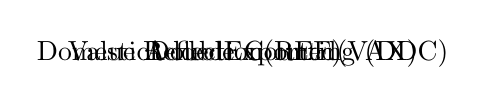
\begin{tikzpicture}
  %Source https://tikz.net/product-architecture/
  %Define the function structure
  \tikzset{
    grow'=right,level distance=25mm, sibling distance =3.5mm,
    execute at begin node=\strut,
    every tree node/.style={
            draw,
            rounded corners,
            anchor = west,
            minimum width=20mm,
            text width=18mm,
            align=center,
            font = {\scriptsize}},
           edge from parent/.style={draw, edge from parent fork right}
  }
  %Draw the function structure (top to bottom)
  %distance from root: width of tree
  \begin{scope}[frontier/.style={distance from root=75mm}]
  \Tree
  [.{Gross \\ Exports \\ (EXGR)}
        [.{Domestic \\ Content \\ (DC)}
            [.{Domestic \\ Value Added \\ (DVA)}
            \node(f1){Value Added \\ Exported \\ (VAX)};
            \node(f2){Reflection \\ (REF)};
            ]
            \node(f4){Domestic \\ Double Counting (DDC)};
        ]
        [.{Foreign Content \\ (FC)}
            [.{Foreign \\ Value Added \\ (FVA)}
            ]
            [.{Foreign \\ Double Counting \\ (FDC)}
            ]
        ]
  ]
  \end{scope}
  \end{tikzpicture}
  \label{fig:decomposition}
\end{figure}

Using these indicators (or parts thereof) we can obtain additional indicators to
measure the participation of countries in global value chains, whether in the
form of foreign inputs used in the domestic production of exports (backward
vertical specialization) or in the form of domestic inputs exported to be used
in the production of foreign exports (forward vertical specialization). In case
these indicators are available, the denomination will be global value chain
participation (GVC), divided in global value chain participation backwards
(GVCB) and forward (GVCF).

\hypertarget{usage-1}{%
\subsection{Usage}\label{usage-1}}

The command \texttt{make\_exvadec()} (export value added decomposition) provides, from a
\texttt{wio} object, the full decomposition of the value added in exports for every
country or for a particular country or country group, according to different
methodologies. The command syntax is as follows:

\begin{verbatim}
make_exvadec(wio_object, exporter = "all", method = "bm_src",
             output = "standard", quiet = TRUE)
\end{verbatim}

with the following arguments:

\begin{itemize}
\tightlist
\item
  \texttt{wio\_object} is an object of class \texttt{wio} obtained through the
  command \texttt{make\_wio}.
\item
  \texttt{exporter} is a string with the code for the exporting country.
  Default is \texttt{"all"} (producing an output of dimension \(GN \times G\)), but
  can be the code of a country, e.g., \texttt{"ESP"}, or country group, e.g.,
  \texttt{"EU27"} (producing an output of dimension \(N \times G\)).
\item
  \texttt{method} is a string specifying the decomposition method.
\item
  \texttt{output} is a string specifying the desired output type.
\item
  \texttt{quiet} is a boolean indicating whether to produce output silently (default is
  \texttt{FALSE}).
\end{itemize}

The available methods and outputs are summarized in Table
\ref{tab:methodoutput}. Selecting \texttt{"bm\_src"} will produce a
Borin and Mancini (2023) source-based decomposition (from our point of view,
the most methodologically sound), \texttt{"bm\_snk"} a Borin and Mancini (2023) sink-based
decomposition, \texttt{"my"} a Miroudot and Ye (2021) decomposition, \texttt{"wwz"} a
Wang, Wei, and Zhu (2013) decomposition, \texttt{"kww"} a Koopman, Wang, and Wei (2014)
decomposition and \texttt{"oecd"} a basic OECD decomposition.

 \begin{table}[h]
  \small
  \centering
  \caption{Output}
  \label{tab:methodoutput}
  \begin{tabular}{llll}
     \hline
     Decomposition & Description & Perimeters & \code{output} options \\
     \code{method} & ~ & (approach/perspective) & ~ \\ \hline
     \code{"bm\_src"} & Borin and Mancini & Source-based /
     & \code{"basic"}, \code{"standard"}, \\
     ~ & (2019) source-based  & various & \code{"terms"} \\ \hline
     \code{"bm\_snk"} & Borin and Mancini & Sink-based /
     & \code{"standard"}, \code{"terms"} \\
     ~ & (2019) sink-based & exporting country & ~ \\ \hline
     \code{"my"} & Miroudot and Ye & Source-based /
     & \code{"standard"}, \code{"terms"} \\
     ~ & (2021) source-based  & various & \code{"terms2"} \\ \hline
     \code{"wwz"} & Wang et al. (2013) & Mix of both
     & \code{"standard"}, \code{"terms"}, \\
     ~ & ~ & ~ & \code{"terms2"} \\ \hline
     \code{"kww"} & Koopman et al. & Sink-based /
     & \code{"standard"}, \code{"terms"}, \\
     ~ & (2014) & mixed & ~ \\ \hline
     \code{"oecd"} & OECD TiVA (not & Not applicable
     & \code{"standard"}, \code{"terms"}, \\
     ~ & a decomposition) & ~ & \code{"tiva"} \\ \hline
  \end{tabular}
\end{table}

The \texttt{"standard"} output of \texttt{make\_exvadec()} will include a series of matrices of
dimension \(GN \times G\) (when exporter is \texttt{"all"}) or of dimension \(N \times G\)
(when the exporting country is specified, e.g., \texttt{"USA"}), with breakdown by
exporting country and sector, and by importer (country of destination), plus
additional metadata:

\begin{itemize}
\tightlist
\item
  \(\mathbf{EXGR}\), total gross exports by country and exporting sector
  and by country of destination.
\item
  \(\mathbf{DC}\), total domestic content in exports by exporting sector
  and country of destination.
\item
  \(\mathbf{DVA}\), domestic value added (including value added that
  returns home).
\item
  \(\mathbf{VAX}\), or value added effectively exported.
\item
  \(\mathbf{REF}\), or reflection, value added that is eventually absorbed
  in the exporting country and therefore does not constitute real exports.
\item
  \(\mathbf{DDC}\), or domestic double counting, or flows of value added
  that are reexported after passing a second time for the exporting country
  and therefore nor constituting real value added.
\item
  \(\mathbf{FC}\), total foreign value added content in exports
  (including double counting).
\item
  \(\mathbf{FVA}\), foreign value added, excluding double counting.
\item
  \(\mathbf{FDC}\), foreign double content, or flows of foreign value added
  that have passed more than once by the exporting country, therefore already
  computed.
\end{itemize}

In some cases, indicators reflecting the participation in global value chains
(vertical specialization) will be provided, mainly foreign value added that
eventually takes part in the domestic production of exports (\(\mathbf{GVCB}\) or
global value chain participation backwards) or domestic value added that
eventually takes part in the foreign production of exports (\(\mathbf{GVCF}\) or
global value chain participation forward).

\texttt{exvadec} objects will inherit metadata of the \texttt{wio} object they come from, like
\texttt{dims}, \texttt{names}, or \texttt{source} (\texttt{type}), plus the indication of the decomposition
\texttt{method} used and, in case of individual decompositions, the \texttt{exporter}. The
\texttt{"standard"} output should be enough for most analyses, but alternative outputs
can be specified with the argument \texttt{output}. The option \texttt{"terms"} will show all
the elements of the decomposition (whose sum is the total value of gross
exports), which is useful if we need to distinguish the value added induced by
intermediate outputs. The Wang, Wei, and Zhu (2013) decomposition corresponds with
the terminology of their Table A2 (pg. 35), but an additional \texttt{"terms2"} is
provided (with the terminology of their Table E1, pg. 61).

The \texttt{"kww"} and \texttt{"wwz"} methods are, in fact, a mix of perspectives and
approaches. The exporting country perspective and the source approach should
probably be considered as the standard, but some alternative approaches (like
the sink approach, considering value added all flows prior to the last border
crossing) and various tailored perspectives are provided. Thus, the sector,
bilateral or bilateral-sector perspectives consider double counting all flows
out of those perimeters, and can be calculated for the \texttt{"bm\_src"} and the \texttt{"my"}
methods (by using the additional arguments \texttt{partner} and \texttt{sector}).
Additionally, the \texttt{"my"} method allows a world perspective (using \texttt{perim\ =\ "WLD"}), consider as double counting the crossing of \emph{any} border more than
once, not only that of the exporting country.

We have included an additional decomposition called \texttt{"oecd"}, which is not a
true full decomposition method, but represents nevertheless a calculation of
several elements of value added in exports. It includes a \texttt{"tiva"} output to
show the most typical indicators included in the OECD TiVA database. In this
decomposition (unlike in the the rest), the bilateral VAX is just VAX absorbed
in the partner country.

\hypertarget{examples}{%
\subsection{Examples}\label{examples}}

To create create a full decomposition of the value added in the exports of Spain
using the method of Borin and Mancini (2023), using a exporting country perspective
and a source-based approach, we would type:

\begin{verbatim}
exvadec <- make_exvadec(wio, exporter = "ESP", method = "bm_src")
\end{verbatim}

\begin{verbatim}
#> ======================================================================
#>        DECOMPOSITION OF VALUE ADDED IN EXPORTS OF SPAIN IN 2022
#>                Sector: All sectors
#>                Destination: All countries
#> ======================================================================
#>  VA_components                              USD_MM  Percent
#>  Gross exports of goods and services (EXGR) 4666.96 100.00 
#>    Domestic Content in VA (DC)              2165.17  46.39 
#>      Domestic Value Added (DVA)             1880.60  40.30 
#>        Value Added Exported (VAX)           1624.18  34.80 
#>        Reflection (REF)                      256.41   5.49 
#>      Domestic Double Counting (DDC)          284.58   6.10 
#>    Foreign Content in VA (FC)               2501.78  53.61 
#>      Foreign Value Added (FVA)              2176.21  46.63 
#>      Foreign Double Counting (FDC)           325.58   6.98 
#>  Global Value Chain-related trade (GVC)     4034.25  86.44 
#>  GVC-related trade, backward (GVCB)         2786.36  59.70 
#>  GVC-related trade, forward (GVCF)          1247.89  26.74 
#> ======================================================================
#> Method: Borin and Mancini (2023), source-based, standard output
#> Country perspective, source approach
\end{verbatim}

If we want to go deeper into the components of this value added,
differentiating between final and intermediate exports, we can use:

\begin{verbatim}
exvadec.terms <- make_exvadec(wio, exporter = "ESP", 
                              method = "bm_src", output = "terms")
\end{verbatim}

\begin{verbatim}
#> ======================================================================
#>        DECOMPOSITION OF VALUE ADDED IN EXPORTS OF SPAIN IN 2022
#>                Sector: All sectors
#>                Destination: All countries
#> ======================================================================
#>  VA_components                               USD_MM  Percent
#>  EXGR (Gross exports of goods and services)  4666.96 100.00 
#>    T01 VAX1 (DVA, finals)                     534.98  11.46 
#>    T02 VAX2 (DVA, interm. for absorption)      97.73   2.09 
#>    T03 VAX3 (DVA, interm. for final exports)  314.51   6.74 
#>    T04 VAX4 (DVA, interm. for reexport)       676.96  14.51 
#>    T05 REF1 (Reflection, finals)              102.25   2.19 
#>    T06 REF2 (Reflection, intermediates)       154.17   3.30 
#>    T07 DDC (Domestic Double Counting)         284.58   6.10 
#>    T08 FVA1 (FVA, finals)                     631.12  13.52 
#>    T09 FVA2 (FVA, interm. for absorption)     112.29   2.41 
#>    T10 FVA3 (FVA, interm. for final exports)  478.65  10.26 
#>    T11 FVA4 (FVA, interm. for reexport)       954.15  20.44 
#>    T12 FDC (Foreign Double Counting)          325.58   6.98 
#> ======================================================================
#> Method: Borin and Mancini (2023), source-based, terms output
#> Country perspective, source approach
\end{verbatim}

If we want to get a list of common trade indicators (exports,
imports, value added, production) similar to those of the TiVA database, we
could just use \texttt{make\_exvadec()} with the method \texttt{"oecd"} and
\texttt{output\ =\ "tiva"}.

\begin{verbatim}
tiva <- make_exvadec(wio, exporter = "ESP", 
                     method = "oecd", output = "tiva")
\end{verbatim}

\begin{verbatim}
#> ======================================================================
#>        DECOMPOSITION OF VALUE ADDED IN EXPORTS OF SPAIN IN 2022
#>                Sector: All sectors
#>                Destination: All countries
#> ======================================================================
#>  VA_components                               USD_MM  Percent
#>  Gross exports of goods and services (EXGR)  4666.96 100.00 
#>    Gross exports, finals (EXGR_FNL)          1343.03  28.78 
#>    Gross exports, intermediates (EXGR_INT)   3323.92  71.22 
#>    Gross imports (IMGR)                      5292.12 113.40 
#>    Gross imports, finals (IMGR_FNL)          2386.14  51.13 
#>    Gross imports, intermediates (IMGR_INT)   2905.98  62.27 
#>    Domestic absorption (DOM)                  739.92  15.85 
#>    Domestic absorption, finals (DOM_FNL)      224.26   4.81 
#>    Domestic absorption, interm. (DOM_INT)     515.66  11.05 
#>    Gross balance (BALGR)                     -625.17 -13.40 
#>    Domestic Content in VA (EXGR_DVA)         2165.17  46.39 
#>    Direct domestic VA content (EXGR_DDC)     1757.25  37.65 
#>    Indirect domestic VA content (EXGR_IDC)    123.34   2.64 
#>    Reimported domestic VA content (EXGR_RIM)  284.58   6.10 
#>    Value Added in final demand (FD_VA)       1985.24  42.54 
#>    DVA in dom. final dem. (VAD) (DXD_DVA)     361.05   7.74 
#>    DVA in foreign final dem. (VAX) (FFD_DVA) 1624.18  34.80 
#>    FVA in dom. final dem. (VAM) (DFD_FVA)    2249.35  48.20 
#>    Balance of VA (VAX - VAM) (BALVAFD)       -625.17 -13.40 
#>    Foreign VA Content (EXGR_FVA)             2501.78  53.61 
#>    Backward participation in GVC (DEXFVAP)   2501.78  53.61 
#>    Forward participation in GVC (FEXDVAP)    3047.87  65.31 
#>    Value added (VA)                          1985.24  42.54 
#>    Production (PROD)                         5406.87 115.85 
#> ======================================================================
#> Method: OECD (2022), TiVA output
#> Country perspective, source approach
\end{verbatim}

\hypertarget{direction-origin-and-destination-of-value-added}{%
\section{Direction (origin and destination) of value added}\label{direction-origin-and-destination-of-value-added}}

The decomposition of \texttt{make\_exvadec()} does not distinguish between the different
sources of foreign value added. This is where the command \texttt{make\_exvadir()} might
be useful. It provides data on the direction of value added, i.e., details of
both the geographical and sectoral origin of the value added incorporated in
exports and of the final destination (in gross terms or in terms of final
demand). It allows therefore a thorough analysis of where the value added is
generated and where it ends up (for instance, how EU services are important for
UK's exports of goods, or the role of China as intermediate party in the exports
of Russia).

\hypertarget{methodology}{%
\subsection{Methodology}\label{methodology}}

The command \texttt{make\_exvadir()} produces an output which is the result of
multiplying the value added matrix \(\hat{\mathbf{V}}\) by the global Leontief
inverse matrix \(\mathbf{B}\) by a matrix of exports \(\mathbf{EXGR}\), but with a
high level of specification of the three matrices. First, the matrix
\(\hat{\mathbf{V}}\) (\(\mathbf{V}\) diagonalized, to preserve the sector
information) will be multiplied by a specific form of \(\mathbf{B}\): regular
\(\mathbf{B}\) to obtain the total value added content, \(\mathbf{B}_d\) to obtain
the domestic value added content and \(\mathbf{B_m}\) to obtain the foreign value
added content; or its equivalents in the form of extraction matrices
\(\mathbf{B}^{xs}\) to obtain the total, domestic or foreign value added excluding
double counting, according to the methodology of
Borin and Mancini (2023).

Then, depending of the sectoral perspective, the product \(\hat{\mathbf{V}} \mathbf{B}\) will be left as it is (sector of origin) or will be summed up by
columns and diagonalized, i.e., as \(\widehat{\mathbf{VB}}\) (default option,
exporting sector perspective). The specification of sectors or countries of
origin of value added will be done by setting the non-specified values to zero.
If the exporter is a group of countries, there is the possibility of considering
intra-regional flows as exports or not (by default, intra-regional flows will be
excluded).

Finally, the resulting adjusted product \({\mathbf{VB}}\) will be multiplied by a
form of export matrix \(\mathbf{EXGR}\). By default, the ordinary gross export
matrix will be considered, but the option will be given to express exports in
terms of absorption (i.e., final demand), as \(\mathbf{EXGRY}\), giving in this
case the possibility of distinguishing between destination of final goods
(\(\mathbf{Y_m}\)) and destination of intermediate exports processed as final
goods (\(\mathbf{A_m B Y}\): this is the only way of calculating the value added
induced by intermediate exports).

Additionally, the possibility will be given to consider exports that go via a
specific country, i.e., an intermediate importer (for example, Russian exports
to the EU that go via China). If this is the case, \(\widehat{\mathbf{VB}}\) will
be multiplied by \(\mathbf{Y}_{sr} + \mathbf{A}_{sr}[\mathbf{BY}]_r\), with \(s\)
being the exporter and \(r\) the intermediate importer, and \([\mathbf{BY}]_r\)
the rows of product \(\mathbf{BY}\) for country \(r\)), i.e., the exports of \(s\)
used in the production of \(r\), that ends up in \(r\) or exported elsewhere.

\hypertarget{usage-2}{%
\subsection{Usage}\label{usage-2}}

The syntax of \texttt{make\_exvadir()} is:

\begin{verbatim}
make_exvadir(wio_object, va_type = "TC", flow_type = "EXGR", exporter,
             via = "any", sec_orig = "all", geo_orig = "all",
             intra = FALSE, perspective = "exporter")
\end{verbatim}

The arguments are as follows:

\begin{itemize}
\tightlist
\item
  \texttt{wio\_object} is an object of class \texttt{wio} (required).
\item
  \texttt{va\_type} is a string describing the type of value added: \texttt{"TC"},
  the default, is the total content in value added (matrix \(\mathbf{B}\)), both
  foreign and domestic, but we can also select \texttt{"DC"} (the domestic value
  added content, using matrix \(\mathbf{B_d}\)) or \texttt{"FC"} (the foreign value
  added content, using matrix \(\mathbf{B_m}\)). \texttt{"TVA"} is the total pure
  value added, i.e., excluding double counting (matrix
  \(\mathbf{B}^{xs}\)), and we can also get the \texttt{"DVA"} (domestic
  value added, excluding double counting, matrix \(\mathbf{B_d}^{xs}\)) or
  the \texttt{"FVA"} (foreign value added, excluding double counting, matrix
  \(\mathbf{B_m}^{xs}\)).
\item
  \texttt{flow\_type} is a string specifying the type of export flow. Default is
  gross total exports (\texttt{"EXGR"}). Alternatives are exports expressed
  in terms of final demand: total exports (\texttt{"EXGRY"}), final exports
  (\texttt{"EXGRY\_FIN"}) or intermediate exports (\texttt{"EXGRY\_INT"}). The latter
  options will show where value added exported is eventually absorbed,
  regardless of where it was initially exported.
\item
  \texttt{exporter} is a string reflecting the code of the exporting country or
  group of countries.
\item
  \texttt{via} is a string with the code of the intermediate importing country or
  country group. Default is \texttt{"any"}. This option requires flows to be expressed
  necessarily in terms of final demand.
\item
  \texttt{geo\_orig} is a string with the code of the country or country group origin
  of value added. Default is \texttt{"all"}.
\item
  \texttt{sec\_orig} is string with the code of sector of origin of value added (e.g.,
  \texttt{"AGR"}, \texttt{"MANUF"}, \texttt{"SRVWC"}\ldots). Default is \texttt{"all"}.
\item
  \texttt{intra} is a boolean to specify whether to include or not intra-region
  exports (default is \texttt{FALSE}, i.e., EU27 exports will include only extra-EU
  exports).
\item
  \texttt{perspective} shows the sectoral perspective of value added. Default is
  exporting sector (\texttt{"exporter"}) but sector of \texttt{"origin"} can also be
  specified.
\end{itemize}

Please note that, compared to \texttt{make\_exvadec()}, \texttt{make\_exvadir()} is logically
more restricted at decomposing value added, so in principle calculations will
be shown in terms of domestic and foreign content (DC/FC) or, at most, domestic
and foreign value added (DVA/FVA, excluding double counting), but including
reflection (REF). Also note that the total content in value added from all
origins and all sectors is, precisely, the value of total gross exports.

\hypertarget{example}{%
\subsection{Example}\label{example}}

We have seen that the foreign content in Spanish exports amounts to USD 2501.78
million. Where does it come from? The specific geographical and sector origin of
the value added in exports can be obtained using the command \texttt{make\_exvadir()}:

\begin{verbatim}
exvadir <- make_exvadir(wio, exporter = "ESP", va_type = "FC", 
                        flow_type = "EXGR")
head(exvadir$FC, 10)
\end{verbatim}

\begin{verbatim}
#>           ESP      FRA      MEX      USA      CHN      ROW
#> ESP_01T09   0  0.00000  0.00000  0.00000  0.00000  0.00000
#> ESP_10T39   0  0.00000  0.00000  0.00000  0.00000  0.00000
#> ESP_41T98   0  0.00000  0.00000  0.00000  0.00000  0.00000
#> FRA_01T09   0 19.45318 26.47295 15.19438 35.51728 24.42115
#> FRA_10T39   0 14.09801 34.93554 23.48504 32.13613 27.09630
#> FRA_41T98   0 15.84674 25.71533 14.12113 17.62330 14.63281
#> MEX_01T09   0 38.41321 52.27477 30.00356 70.13415 48.22319
#> MEX_10T39   0 31.07698 77.01024 51.76931 70.83935 59.72978
#> MEX_41T98   0 33.18999 53.85912 29.57581 36.91088 30.64749
#> USA_01T09   0 23.35813 31.78700 18.24443 42.64685 29.32333
\end{verbatim}

Note that the \texttt{exvadir} object that we have obtained is different from
the \texttt{exvadec} object, in the sense that `exporters' in an \texttt{exvadir}
object are the different countries and sectors of origin of the value added
included in the exports of a specific country (in this case, Spain). We can
better understand this by typing \texttt{summary(exvadir)}:

\begin{verbatim}
summary(exvadir)
\end{verbatim}

\begin{verbatim}
#> 
#> ====================================================================== 
#>   ORIGIN AND DESTINATION OF VALUE ADDED IN EXPORTS OF SPAIN IN 2022 
#> ====================================================================== 
#> Value added type: Foreign VA content (FC) 
#> In type of flow: Total gross exports (EXGR) 
#> That goes via country: any 
#> Using inputs from sector: all sectors 
#> Of country: all countries 
#> With sector perspective: exporter 
#> ====================================================================== 
#> 
#> Available countries of origin of VA (G): 6 
#> ESP, FRA, MEX, USA, CHN, ROW 
#>  
#> Available sectors of origin of VA (N): 3 
#> D01T09, D10T39, D41T98 
#>  
#> Available destinations of VA (G): 6 
#> ESP, FRA, MEX, USA, CHN, ROW 
#> 
\end{verbatim}

Now we will see how to maximize the information given by these objects.

\hypertarget{sector-and-geographic-analysis}{%
\section{Sector and geographic analysis}\label{sector-and-geographic-analysis}}

The commands \texttt{make\_wio()}, \texttt{make\_exvadec()} and \texttt{make\_exvadir()}
produce objects that are lists of matrices will a full breakdown by sector and
countries of destination. However, most analyses require grouping of those
variables. The advantage is that grouping by sector or by destination do not
require additional computing, just an aggregation of variables.

To check the information about sectors, it suffices to print \texttt{info\_sec()}:

\begin{verbatim}
info_sec("iciotest")
\end{verbatim}

\begin{verbatim}
#> 
#> ======================================================================
#>  Test Input Output Table, ICIO-type, 2022 edition
#> ======================================================================
#> 
#> Individual sectors:
#> PRIMARY: D01T09 (Primary sector), MANUF: D10T39 (Manufacturing),
#> SRVWC: D41T98 (Services, including construction)
#> 
#> Sector groups:
#> TOTAL: D01T98 (Total goods and services), GOODSWU: D01T39 (Goods,
#> total, incl. utilities)
\end{verbatim}

To check the information about available countries, the command is
\texttt{info\_geo()}:

\begin{verbatim}
info_geo("iciotest")
\end{verbatim}

\begin{verbatim}
#> 
#> ======================================================================
#>  Test Input Output Table, ICIO-type, 2022 edition
#> ======================================================================
#> 
#> Individual countries:
#> FRA (France), MEX (Mexico), ESP (Spain), USA (United States), CHN
#> (China), ROW (Rest of the world)
#> 
#> Groups of countries:
#> WLD (World), EU27 (EU-27), NONEU27 (Non-EU27), NAFTA (NAFTA), USMCA
#> (USMCA)
\end{verbatim}

These commands do not require to have a \texttt{wio} in the environment, so we
can just check what countries are available in the OECD's ICIO tables, 2023
edition.

\begin{verbatim}
info_geo("icio2023")
\end{verbatim}

\begin{verbatim}
#> 
#> ======================================================================
#>  OECD's Inter-Country Input-Output Table (ICIO), 2023 edition
#> ======================================================================
#> 
#> Individual countries:
#> AUS (Australia), AUT (Austria), BEL (Belgium), CAN (Canada), CHL
#> (Chile), CZE (Czech Republic), DNK (Denmark), EST (Estonia), FIN
#> (Finland), FRA (France), DEU (Germany), GRC (Greece), HUN (Hungary),
#> ISL (Iceland), IRL (Ireland), ISR (Israel), ITA (Italy), JPN (Japan),
#> KOR (Korea), LVA (Latvia), LTU (Lithuania), LUX (Luxembourg), MEX
#> (Mexico), NLD (Netherlands), NZL (New Zealand), NOR (Norway), POL
#> (Poland), PRT (Portugal), SVK (Slovak Republic), SVN (Slovenia), ESP
#> (Spain), SWE (Sweden), CHE (Switzerland), TUR (Turkey), GBR (United
#> Kingdom), USA (United States), ARG (Argentina), BGD (Bangladesh), BLR
#> (Belarus), BRA (Brazil), BRN (Brunei Darussalam), BGR (Bulgaria), KHM
#> (Cambodia), CMR (Cameroon), CHN (China), COL (Colombia), CRI (Costa
#> Rica), CIV (Côte d'Ivoire), HRV (Croatia), CYP (Cyprus), EGY (Egypt),
#> IND (India), IDN (Indonesia), JOR (Jordania), HKG (Hong Kong, China),
#> KAZ (Kazakhstan), LAO (Laos), MYS (Malaysia), MLT (Malta), MAR
#> (Morocco), MMR (Myanmar), NGA (Nigeria), PAK (Pakistan), PER (Peru),
#> PHL (Philippines), ROU (Romania), RUS (Russia), SAU (Saudi Arabia),
#> SEN (Senegal), SGP (Singapore), ZAF (South Africa), TWN (Chinese
#> Taipei), THA (Thailand), TUN (Tunisia), UKR (Ukraine), VNM (Vietnam),
#> ROW (Rest of the world)
#> 
#> Groups of countries:
#> WLD (World), EU28 (EU-28), EU27 (EU-27), OECD (OECD), EMU (EMU),
#> NONEU28 (Non-EU28), NONEU27 (Non-EU27), NONOECD (Non-OECD),
#> EU28NONEMU (EU-28 not EMU), EU27NONEMU (EU-27 not EMU), EURNONEU
#> (Rest of Europe), EUROPE (Europe), AMER (America), NAMER (North
#> America), CSAMER (Central and South America), LATAM (Latin America
#> and Caribbean), AFRI (Africa), ASIA (Asia), OCEA (Oceania), ASIAOC
#> (Asia and Oceania), G20 (G-20), G7 (G7), NAFTA (NAFTA), USMCA
#> (USMCA), EEA (EEA), EFTA (EFTA), APEC (APEC), ASEAN (ASEAN), RCEP
#> (RCEP)
\end{verbatim}

Additionally, the commands \texttt{get\_geo\_codes()} and \texttt{get\_sec\_codes()}
provide details about the components of the different groups. These commands
are also directly applicable for any available input-output table. For
instance, for \texttt{"wiod2016"} we would have the following components of
NAFTA:

\begin{verbatim}
get_geo_codes("NAFTA", wiotype = "wiod2016")
\end{verbatim}

\begin{verbatim}
#> [1] "CAN|MEX|USA"
\end{verbatim}

And for \texttt{"icio2023"} we have the following components of the information
services sector (\texttt{INFO}):

\begin{verbatim}
get_sec_codes("INFO", wiotype = "icio2023")
\end{verbatim}

\begin{verbatim}
#> [1] "D58T60|D61|D62T63"
\end{verbatim}

Once we know the sector and geographical disaggregation, we can discuss
how to take advantage of the information contained in \texttt{exvatools} objects.

\hypertarget{breaking-down-decompositions}{%
\section{Breaking down decompositions}\label{breaking-down-decompositions}}

Once we have obtained a decomposition, we can play with the results in terms of
sectors and countries of destination just using the command
\texttt{get\_exvadec\_bkdown()}. For instance, to select the value added in Spanish
exports of services (including construction) to the United States, we just have
to type:

\begin{verbatim}
get_exvadec_bkdown(exvadec, exporter = "ESP", 
                   sector = "SRVWC", importer = "USA")
\end{verbatim}

\begin{verbatim}
#> ======================================================================
#>        DECOMPOSITION OF VALUE ADDED IN EXPORTS OF SPAIN IN 2022
#>                Sector: Services, including construction (SRVWC)
#>                Destination: United States (USA)
#> ======================================================================
#>  VA_components                              USD_MM Percent
#>  Gross exports of goods and services (EXGR) 276.71 100.00 
#>    Domestic Content in VA (DC)              159.63  57.69 
#>      Domestic Value Added (DVA)             145.95  52.74 
#>        Value Added Exported (VAX)           127.28  46.00 
#>        Reflection (REF)                      18.67   6.75 
#>      Domestic Double Counting (DDC)          13.68   4.94 
#>    Foreign Content in VA (FC)               117.08  42.31 
#>      Foreign Value Added (FVA)              101.53  36.69 
#>      Foreign Double Counting (FDC)           15.55   5.62 
#>  Global Value Chain-related trade (GVC)     221.62  80.09 
#>  GVC-related trade, backward (GVCB)         130.76  47.26 
#>  GVC-related trade, forward (GVCF)           90.86  32.84 
#> ======================================================================
#> Method: Borin and Mancini (2023), source-based, standard output
#> Country perspective, source approach
\end{verbatim}

Note that the bilateral \texttt{VAX} in this case shows the value added exported to
the United States, regardless of the final absorption country.

We can also produce an \texttt{exvadec} object will all countries and then select any
exporting country and any partner or sector:

\begin{verbatim}
exvadec.all <- make_exvadec(wio, exporter = "all", quiet = TRUE)
\end{verbatim}

and then:

\begin{verbatim}
get_exvadec_bkdown(exvadec.all, exporter = "USA", 
                   sector = "MANUF", importer = "CHN")
\end{verbatim}

\begin{verbatim}
#> ======================================================================
#>    DECOMPOSITION OF VALUE ADDED IN EXPORTS OF UNITED STATES IN 2022
#>                Sector: Manufacturing (MANUF)
#>                Destination: China (CHN)
#> ======================================================================
#>  VA_components                              USD_MM Percent
#>  Gross exports of goods and services (EXGR) 400.89 100.00 
#>    Domestic Content in VA (DC)              164.19  40.96 
#>      Domestic Value Added (DVA)             138.36  34.51 
#>        Value Added Exported (VAX)           114.29  28.51 
#>        Reflection (REF)                      24.06   6.00 
#>      Domestic Double Counting (DDC)          25.83   6.44 
#>    Foreign Content in VA (FC)               236.70  59.04 
#>      Foreign Value Added (FVA)              204.59  51.03 
#>      Foreign Double Counting (FDC)           32.12   8.01 
#>  Global Value Chain-related trade (GVC)     379.14  94.58 
#>  GVC-related trade, backward (GVCB)         262.53  65.49 
#>  GVC-related trade, forward (GVCF)          116.61  29.09 
#> ======================================================================
#> Method: Borin and Mancini (2023), source-based, standard output
#> Country perspective, source approach
\end{verbatim}

Apart from the console printout, \texttt{get\_exvadec\_bkdown()} will output a
matrix with the results.

\hypertarget{extracting-data-from-exvatools-objects}{%
\section{Extracting data from exvatools objects}\label{extracting-data-from-exvatools-objects}}

The command \texttt{get\_data()} takes an \texttt{exvatools} object (\texttt{wio} or
\texttt{exvadec}) and produces a value or a matrix of values. It allows a quick
extraction of data. The main advantage of \texttt{get\_data()} is that it does not
only admit individual sectoral codes (\texttt{"MANUF"}) or destination country
codes (\texttt{"USA"}, \texttt{"NAFTA"}), but also lists of sectors and countries
in vector form. Therefore, we can easily produce a matrix of domestic value
added with breakdown by sector and by destination groups. The syntax of
\texttt{get\_data()}is as follows:

\begin{verbatim}
get_data(exvatools_object, variable, exporter = NULL,
         sector = "TOTAL", importer = "WLD", custom = FALSE)
\end{verbatim}

The arguments are as follows:

\begin{itemize}
\tightlist
\item
  \texttt{exvatools\_object} (required) is an object of class \texttt{wio}, \texttt{exvadec} or
  \texttt{exvadir}, and \texttt{variable} is a string specifying one of the variables included
  in the \texttt{exvatools\_object}, such as \texttt{"EXGR"}, \texttt{"VAX"}, \texttt{"FVA"}, etc.
\item
  \texttt{exporter} is a string vector with one or more codes of exporters or groups of
  exporters, such as \texttt{"ESP"}, \texttt{"EU27"}, \texttt{c("WLD",\ "EU27",\ "NONEU27")}, etc. This
  will define the rows in the resulting matrix. Specific exclusions can be
  accepted through the excluding code \texttt{x} (lowercase x), so \texttt{"EU27xESP"} would
  be EU countries, excluding Spain, \texttt{"WLDxEU27"} would be total world except EU,
  and so on. More than one exception can be specified with the \texttt{"\textbar{}"} element,
  such as in \texttt{"WLDxESP\textbar{}FRA\textbar{}ITA"}. Available countries and country group id codes
  can be checked with the command \texttt{info\_geo()}. The argument \texttt{exporter} is
  required in all cases except two: in case of a country-specific \texttt{exvadec}
  object, in which the exporter is previously defined, and in case of an
  \texttt{exvadir} object, where, by definition, there is only one exporter. Note that,
  in the case of an \texttt{exvadir} object obtained for country \(s\), the argument
  \texttt{exporter} does not refer to country \(s\) itself, but to the \(t = 1 \dots G\)
  exporters of value added that is used by country \(s\) to produce its exports.
  Therefore, if the \texttt{exporter} argument is missing, the default behavior of
  \texttt{get\_data()} will be different, depending on the case: for a country-specific
  \texttt{exvadec}, it will default to the exporting country, whereas for an \texttt{exvadir}
  object it will default to \texttt{"WLD"} (i.e., sum of all origins of value added).
\item
  \texttt{sector} is a string vector with one or more codes of sectors or groups
  of sectors, such as \texttt{"MANUF"}, \texttt{"SERVS"}, \texttt{"TOTAL"},
  \texttt{c("TOTAL",\ "GOODSWU",\ "SRVWC")}, etc. These will also show as rows in
  the result. Specific exclusions can be accepted through the excluding code
  \texttt{x}, so \texttt{"MANUFxPET"} would be manufactures, excluding oil products,
  \texttt{"SRVWCxBIZSV"} would be total services (with construction) except
  business services, and so on. Available sector id codes can be checked with
  the command \texttt{info\_sec()}. Default option is \texttt{"TOTAL"} (sum of all
  sectors for the specific exporter). The option \texttt{"all"} can be used to
  specify all sectors.
\item
  \texttt{importer} is a character string or vector with one or more codes of
  importing countries or groups of countries, such as \texttt{"ESP"},
  \texttt{"EU27"}, \texttt{c("WLD",\ "EU27",\ "NONEU27")}, etc. This defines the
  columns of the result. Default option is \texttt{"WLD"}, i.e, the sum of all
  importers for the specific exporter (and sector) selection.
\item
  \texttt{custom} is a boolean specifying whether custom-made groups of countries
  or sectors present in the environment should be looked up by \texttt{get\_data()}.
  For instance, \texttt{HITECH} could be a specific variable including all
  high-tech sectors, or \texttt{LDC} could be a list of least-developed countries.
  Custom variables should be referred to as strings in \texttt{get\_data()}, so, for
  instance, \texttt{get\_data(exva,\ "VAX",\ exporter\ =\ "LDC",\ custom\ =\ TRUE)} would
  look for a variable called \texttt{LDC} in the environment and would use its
  codes to extract and group data.
\end{itemize}

We can use \texttt{get\_data()} to summarize the foreign content of Spanish
exports, with a breakdown between EU and Non-EU origin (specifying a few
countries) and also distinguishing between goods (with utilities) and
services. We can also break down the destination of those exports between EU
and non-EU countries:

\begin{verbatim}
get_data(exvadir, exporter = c("WLD", "EU27", "FRA",
                               "NONEU27", "USA"),
         sector = c("TOTAL", "GOODSWU", "SRVWC"),
         importer = c("WLD", "EU27", "NONEU27"))
\end{verbatim}

\begin{verbatim}
#>                        WLD      EU27    NONEU27
#> WLD_TOTAL       2501.78421 367.55781 2134.22640
#> WLD_GOODSWU     1772.66226 236.16941 1536.49285
#> WLD_SRVWC        729.12195 131.38840  597.73355
#> EU27_TOTAL       340.74928  49.39794  291.35134
#> EU27_GOODSWU     252.80996  33.55120  219.25877
#> EU27_SRVWC        87.93932  15.84674   72.09258
#> FRA_TOTAL        340.74928  49.39794  291.35134
#> FRA_GOODSWU      252.80996  33.55120  219.25877
#> FRA_SRVWC         87.93932  15.84674   72.09258
#> NONEU27_TOTAL   2161.03493 318.15987 1842.87505
#> NONEU27_GOODSWU 1519.85229 202.61821 1317.23408
#> NONEU27_SRVWC    641.18263 115.54166  525.64097
#> USA_TOTAL        433.65389  64.94868  368.70521
#> USA_GOODSWU      286.90179  38.50383  248.39796
#> USA_SRVWC        146.75210  26.44485  120.30725
\end{verbatim}

If there is not a specific group in the database of sectors or countries,
the user has two options: to create a group and use \texttt{get\_data()} with the
option \texttt{custom\ =\ TRUE}, or simply to use a combination of countries or
sectors with a vertical line \texttt{"\textbar{}"}.

In the latter case, for instance, if we want to combine \texttt{ESP} and \texttt{MEX}
in a single group, we can just type:

\begin{verbatim}
get_data(exvadec.all, "VAX", exporter = "ESP|MEX", 
         sector = c("TOTAL", "MANUF", "SRVWC"), 
         importer = "USA")
\end{verbatim}

\begin{verbatim}
#>                    USA
#> ESP|MEX_TOTAL 756.1258
#> ESP|MEX_MANUF 251.3334
#> ESP|MEX_SRVWC 257.0910
\end{verbatim}

If the vertical line \texttt{"\textbar{}"} is used to join, the exception marker is \texttt{"x"}. It
allows us, for instance, to calculate NAFTA exports, both intra-regional and
extra-regional, employing services and non-services, using as extra-regional
\texttt{"WLDxNAFTA"} and as non-services \texttt{"TOTALxSRVWC"}

\begin{verbatim}
get_data(exvadec.all, "EXGR", exporter = "NAFTA", 
         sector = c("TOTAL", "TOTALxSRVWC", "SRVWC"), 
         importer = c("WLD", "NAFTA", "WLDxNAFTA"))
\end{verbatim}

\begin{verbatim}
#>                         WLD    NAFTA WLDxNAFTA
#> NAFTA_TOTAL       13087.740 2602.338 10485.402
#> NAFTA_TOTALxSRVWC  8736.552 1502.340  7234.212
#> NAFTA_SRVWC        4351.188 1099.998  3251.189
\end{verbatim}

Let us use \texttt{get\_data()}to calculate the relative comparative advantage (RCA) in
terms of gross exports and compare it with that in terms of VAX. The RCA is
the relation between the proportion of exports of sector \(i\) in country \(s\)
to total exports of \(s\) (\(E_{si}/E_s\)) and the proportion of world exports of
sector \(i\) to total world exports (\(E_{wi}/E_w\)). If RCA is more than 1, it
means that country \(s\) has a relative specialization (and a comparative
advantage) in sector \(i%
\) compared to the world average.

We will create a function to calculate the RCA so it can be used with both
gross exports (\texttt{EXGR}) and value added exported (\texttt{VAX}). As we can see,
\texttt{get\_data()} considerably simplifies the calculation of country exports
and sector exports.

\begin{verbatim}
RCA <- function(exva, exvar) {
  Esi <- get_data(exva, exvar, exporter = "all", sector = "all")
  Es <- get_data(exva, exvar, exporter = "all", sector = "TOTAL")
  Es <- rep(as.numeric(Es), each = exva$dims$N)
  Ewi <- get_data(exva, exvar, exporter = "WLD", sector = "all")
  Ewi <- rep(as.numeric(Ewi), exva$dims$G)
  Ew <- as.numeric(get_data(exva, exvar, exporter = "WLD", sector = "TOTAL"))
  rca <- (Esi/Es)/(Ewi/Ew)
  colnames(rca) <- paste0("RCA", ".", exvar)
  return(rca)
}
head(cbind(RCA(exvadec.all, "EXGR"),
           RCA(exvadec.all, "VAX")), 10)
\end{verbatim}

\begin{verbatim}
#>            RCA.EXGR   RCA.VAX
#> ESP_01T09 0.7981206 0.4575154
#> ESP_10T39 1.1110328 1.0953243
#> ESP_41T98 1.0883393 1.3971980
#> FRA_01T09 1.0378051 0.7268141
#> FRA_10T39 1.0686493 1.1512224
#> FRA_41T98 0.8963249 1.0970064
#> MEX_01T09 1.0752922 1.3324652
#> MEX_10T39 0.9908369 1.0324864
#> MEX_41T98 0.9356388 0.6658469
#> USA_01T09 1.0464957 1.2057567
\end{verbatim}

We can see that some relative advantage (RCA \textgreater{} 1) in terms of gross exports
disappear when calculated in terms of VAX, while some other appear.

Another useful application is the calculation of bilateral balances. We can
see that there are considerable difference in bilateral balances when
calculated in terms of value added compared to the same balances using gross
exports.

\begin{verbatim}
EXGR <- get_data(exvadec.all, "EXGR", "all", importer = "all")
IMGR <- bkt(EXGR)
VAX <- get_data(exvadec.all, "VAX", "all", importer = "all")
VAM <- bkt(VAX)
BALGR <- round(EXGR - IMGR, 0)
BALVA <- round(VAX - VAM, 0)
as.data.frame(cbind(BALGR, " "=" ", BALVA),
              row.names = exvadec.all$names$g_names)
\end{verbatim}

\begin{verbatim}
#>     ESP  FRA  MEX  USA  CHN ROW    ESP FRA  MEX  USA  CHN ROW
#> ESP   0    8 -394 -130 -158  49      0  30 -151  -34  -92 111
#> FRA  -8    0   53 -290 -544 173    -30   0  -28 -127 -253  96
#> MEX 394  -53    0  263  189 459    151  28    0   84   68 279
#> USA 130  290 -263    0 -570 -19     34 127  -84    0 -297  74
#> CHN 158  544 -189  570    0 464     92 253  -68  297    0 319
#> ROW -49 -173 -459   19 -464   0   -111 -96 -279  -74 -319   0
\end{verbatim}

\hypertarget{other-useful-commands}{%
\section{Other useful commands}\label{other-useful-commands}}

\CRANpkg{exvatools} provides several additional commands, some of them
resulting from the mere combination of \texttt{make\_exvadir()} and \texttt{get\_data()} with
specific default arguments. Of course, it would be easy to create other custom combinations.

\hypertarget{detailed-origin-of-value-added}{%
\subsection{Detailed origin of value added}\label{detailed-origin-of-value-added}}

The command \texttt{get\_va\_exgr()} provides a detailed sector and geographical origin
and destination of value added.

\begin{verbatim}
get_va_exgr(wio_object, va_type = "FC", 
            geo_orig = "all", sec_orig = "TOTAL",
            geo_export, sec_export = "TOTAL", as_numeric = TRUE)
\end{verbatim}

It allows to analyze, for instance, the percentage of services (both domestic
and foreign) embedded in Spanish exports of manufactures, i.e.~the so-called
`servicification' of Spanish exports:

\begin{verbatim}
get_va_exgr(wio, va_type = "TC", 
            geo_orig = c("ESP", "WLDxESP"), sec_orig = "SRVWC",
            geo_export = "ESP", sec_export = "MANUF", 
            as_numeric = FALSE)
\end{verbatim}

\begin{verbatim}
#>                     WLD
#> ESP_MANUF      84.95594
#> WLDxESP_MANUF 263.71717
\end{verbatim}

On the other hand, if we wanted the value added in services of the US
incorporated in the Spanish exports of manufactures, i.e., the Spanish
dependence of US services to produce exports of manufactures:

\begin{verbatim}
get_va_exgr(wio, geo_orig = "USA", sec_orig = "SRVWC",
            geo_export = "ESP", sec_export = "MANUF")
\end{verbatim}

\begin{verbatim}
#> [1] 51.31605
\end{verbatim}

\hypertarget{detailed-final-absorption-of-value-added}{%
\subsection{Detailed final absorption of value added}\label{detailed-final-absorption-of-value-added}}

Sometimes we are not only interested in the origin, but also in the country of
final absorption. For that we have the command \texttt{get\_va\_exgry()}. This is
equivalent to the OECD's Gross Exports by Origin of Value Added and Final
destination (\texttt{FD\_EXGR\_VA}, \texttt{FD\_EXGRFNL\_VA} and \texttt{FD\_EXGRINT\_VA}), but with much
more flexible geographical and sector options. Since the OECD TiVA database no
longer provides this indicator in their online version, this command becomes
particularly useful.

\begin{verbatim}
get_va_exgry(wio_object, va_type = "TC", flow_type = "EXGRY",
             geo_orig = "WLD", geo_export, sec_export = "TOTAL",
             geo_fd = "WLD", as_numeric = TRUE)
\end{verbatim}

Here \texttt{flow\_type} are exports (expressed in terms of final demand), whether
total (\texttt{"EXGRY"}), final (\texttt{"EXGRY\_FIN"}) or intermediate (\texttt{"EXGRY\_INT"}), and
\texttt{geo\_fd} is the country or region of final demand.

This allows, for instance, to calculate what part of US value added incorporated
in China's exports of manufactures ends up absorbed back in the US.

\begin{verbatim}
get_va_exgry(wio, geo_orig = "USA", geo_export = "CHN",
             sec_export = "MANUF", geo_fd = "USA")
\end{verbatim}

\begin{verbatim}
#> [1] 53.81984
\end{verbatim}

\hypertarget{value-added-induced-by-final-demand}{%
\subsection{Value added induced by final demand}\label{value-added-induced-by-final-demand}}

\CRANpkg{exvatools} also provides a simple command to obtain details of both the
geographical and sector origin of the value added incorporated in exports
induced by final demand.

\begin{verbatim}
get_va_fd(wio_object, va_type = "TOTAL",
          geo_orig = "WLD", sec_orig = "TOTAL",
          geo_fd = "WLD", sec_fd = "TOTAL", intra = FALSE)
\end{verbatim}

This would allow, for instance, the calculation of the Chinese
total value added (or GDP) induced by US final demand for manufactures:

\begin{verbatim}
get_va_fd(wio, geo_orig = "CHN", sec_orig = "TOTAL",
          geo_fd = "USA", sec_fd = "MANUF")
\end{verbatim}

\begin{verbatim}
#>               WLD
#> CHN_TOTAL 229.385
\end{verbatim}

\hypertarget{summary-and-conclusions}{%
\section{Summary and conclusions}\label{summary-and-conclusions}}

We have presented the package \CRANpkg{exvatools} for decomposition of value
added in exports using international-input out tables in \textbf{R}.
\CRANpkg{exvatools} provides a convenient tool for calculating and manipulating
international input-output matrices, and simplifies the decomposition of value
added in exports (using alternative methodologies). It also allows a
straightforward calculation of custom value added indicators.

The purpose of \CRANpkg{exvatools} is to provide the scientific community with
tools to take advantage of the valuable statistical resources that are the
international input-output tables, facilitating the analysis of the complex
interaction between trade in goods and services and between economic sectors in
different countries.

\hypertarget{references}{%
\section*{References}\label{references}}
\addcontentsline{toc}{section}{References}

\hypertarget{refs}{}
\begin{CSLReferences}{1}{0}
\leavevmode\vadjust pre{\hypertarget{ref-arto_measuring_2019}{}}%
Arto, Iñaki, Erik Dietzenbacher, José Manuel Rueda-Cantuche, European Commission, and Joint Research Centre. 2019. {``Measuring {Bilateral} {Trade} in {Terms} of {Value} {Added}.''} JRC Technical Report. \url{https://doi.org/10.2760/639612}.

\leavevmode\vadjust pre{\hypertarget{ref-asian_development_bank_multiregional_2023}{}}%
Asian Development Bank. 2023. {``Multiregional {Input}-{Output} {Database} ({ADB-MRIO}).''} \url{https://kidb.adb.org/mrio}.

\leavevmode\vadjust pre{\hypertarget{ref-belotti_icio_2021}{}}%
Belotti, Federico, Alessandro Borin, and Michele Mancini. 2021. {``Icio: {Economic} Analysis with Intercountry Input--Output Tables.''} \emph{The Stata Journal} 21 (3): 708--55. \url{https://doi.org/10.1177/1536867X211045573}.

\leavevmode\vadjust pre{\hypertarget{ref-borin_measuring_2023}{}}%
Borin, Alessandro, and Michele Mancini. 2023. {``Measuring What Matters in Value-Added Trade.''} \emph{Economic Systems Research}, January, 1--28. \url{https://doi.org/10.1080/09535314.2022.2153221}.

\leavevmode\vadjust pre{\hypertarget{ref-daudin_who_2011}{}}%
Daudin, Guillaume, Christine Rifflart, and Danielle Schweisguth. 2011. {``Who Produces for Whom in the World Economy?''} \emph{Canadian Journal of Economics} 44 (4): 1403--37. \url{https://doi.org/10.1111/j.1540-5982.2011.01679.x}.

\leavevmode\vadjust pre{\hypertarget{ref-foster-mcgregor_value_2013}{}}%
Foster-McGregor, Neil, and Robert Stehrer. 2013. {``Value Added Content of Trade: {A} Comprehensive Approach.''} \emph{Economics Letters} 120 (2): 354--57. \url{https://doi.org/10.1016/j.econlet.2013.05.003}.

\leavevmode\vadjust pre{\hypertarget{ref-johnson_measuring_2018}{}}%
Johnson, Robert C. 2018. {``Measuring {Global} {Value} {Chains}.''} \emph{Annual Review of Economics} 10 (1): 207--36. \url{https://doi.org/10.1146/annurev-economics-080217-053600}.

\leavevmode\vadjust pre{\hypertarget{ref-johnson_accounting_2012}{}}%
Johnson, Robert C., and Guillermo Noguera. 2012. {``Accounting for Intermediates: {Production} Sharing and Trade in Value Added.''} \emph{Journal of International Economics} 86 (2): 224--36. \url{https://doi.org/10.1016/j.jinteco.2011.10.003}.

\leavevmode\vadjust pre{\hypertarget{ref-koopman_tracing_2014}{}}%
Koopman, Robert, Zhi Wang, and Shang-Jin Wei. 2014. {``Tracing {Value}-{Added} and {Double} {Counting} in {Gross} {Exports}.''} \emph{American Economic Review} 104 (2): 459--94. \url{https://doi.org/10.1257/aer.104.2.459}.

\leavevmode\vadjust pre{\hypertarget{ref-lenzen_building_2013}{}}%
Lenzen, Manfred, Daniel Moran, Keiichiro Kanemoto, and Arne Geschke. 2013. {``Building {Eora}: {A} {Global} {Multi}-{Region} {Input}--{Output} {Database} at {High} {Country} and {Sector} {Resolution}.''} \emph{Economic Systems Research} 25 (1): 20--49. \url{https://doi.org/10.1080/09535314.2013.769938}.

\leavevmode\vadjust pre{\hypertarget{ref-leontief_quantitative_1936}{}}%
Leontief, Wassily W. 1936. {``Quantitative {Input} and {Output} {Relations} in the {Economic} {System} of the {United} {States}.''} \emph{Review of Economics and Statistics} 18: 105--25.

\leavevmode\vadjust pre{\hypertarget{ref-los_measuring_2018}{}}%
Los, Bart, and Marcel P. Timmer. 2018. {``Measuring {Bilateral} {Exports} of {Value} {Added}: {A} {Unified} {Framework}.''} NBER Working Paper w24896. NBER. \url{https://doi.org/10.3386/w24896}.

\leavevmode\vadjust pre{\hypertarget{ref-los_tracing_2016}{}}%
Los, Bart, Marcel P. Timmer, and Gaaitzen J. de Vries. 2016. {``Tracing {Value}-{Added} and {Double} {Counting} in {Gross} {Exports}: {Comment}.''} \emph{American Economic Review} 106 (7): 1958--66. \url{https://doi.org/10.1257/aer.20140883}.

\leavevmode\vadjust pre{\hypertarget{ref-miroudot_decomposing_2021}{}}%
Miroudot, Sébastien, and Ming Ye. 2021. {``Decomposing {Value} {Added} in {Gross} {Exports}.''} \emph{Economic Systems Research} 33 (1): 67--87. \url{https://doi.org/10.1080/09535314.2020.1730308}.

\leavevmode\vadjust pre{\hypertarget{ref-nagengast_accounting_2016}{}}%
Nagengast, Arne J., and Robert Stehrer. 2016. {``Accounting for the {Differences} {Between} {Gross} and {Value} {Added} {Trade} {Balances}.''} \emph{The World Economy} 39 (9): 1276--306. \url{https://doi.org/10.1111/twec.12401}.

\leavevmode\vadjust pre{\hypertarget{ref-oecd_oecd_2023}{}}%
OECD. 2023. {``{OECD} {Inter}-{Country} {Input}-{Output} {Database}.''} \url{http://oe.cd/icio}.

\leavevmode\vadjust pre{\hypertarget{ref-quast_decompr_2015}{}}%
Quast, Bastiaan, and Victor Kummritz. 2015. {``Decompr: {Global} {Value} {Chain} {Decomposition} in {R}.''} CTEI Papers 2015-01. Centre for Trade \& Economic Integration. \url{https://qua.st/decompr/}.

\leavevmode\vadjust pre{\hypertarget{ref-remond-tierrez_eu_2019}{}}%
Remond-Tierrez, Isabelle, and José Manuel Rueda-Cantuche, eds. 2019. \emph{{EU} Inter-Country Supply, Use and Input-Output Tables: Full International and Global Accounts for Research in Input Output Analysis ({FIGARO}): 2019 Edition.} LU: EU Publications Office. \url{https://doi.org/10.2785/008780}.

\leavevmode\vadjust pre{\hypertarget{ref-statacorp_stata_2021}{}}%
StataCorp. 2021. {``Stata {Statistical} {Software}: {Release} 17.''} College Station, TX: StataCorp LLC.

\leavevmode\vadjust pre{\hypertarget{ref-timmer_illustrated_2015}{}}%
Timmer, Marcel P., Erik Dietzenbacher, Bart Los, Robert Stehrer, and Gaaitzen J. de Vries. 2015. {``An {Illustrated} {User} {Guide} to the {World} {Input}-{Output} {Database}: The {Case} of {Global} {Automotive} {Production}.''} \emph{Review of International Economics} 23 (3): 575--605. \url{https://doi.org/10.1111/roie.12178}.

\leavevmode\vadjust pre{\hypertarget{ref-wade_ioanalysis_2020}{}}%
Wade, John, and Ignacio Sarmiento-Barbieri. 2020. {``Ioanalysis: {Input} {Output} {Analysis}.''} \url{https://cran.r-project.org/web/packages/ioanalysis/ioanalysis.pdf}.

\leavevmode\vadjust pre{\hypertarget{ref-wang_quantifying_2013}{}}%
Wang, Zhi, Shang-Jin Wei, and Kunfu Zhu. 2013. {``Quantifying {International} {Production} {Sharing} at the {Bilateral} and {Sector} {Levels}.''} NBER Working Paper 19677. National Bureau of Economic Research, Inc. \url{https://econpapers.repec.org/paper/nbrnberwo/19677.htm}.

\end{CSLReferences}

\bibliography{exvatools.bib}

\address{%
Enrique Feás\\
Universidad de Alcalá and Elcano Royal Institute\\%
Universidad de Alcalá, Pl. de San Diego, s/n, 28801 Alcalá de Henares, Madrid, Spain\\ Elcano Royal Institute, Calle del Príncipe de Vergara, 51. 28006 Madrid, Spain\\
%
%
\textit{ORCiD: \href{https://orcid.org/0000-0002-9431-6051}{0000-0002-9431-6051}}\\%
\href{mailto:enrique.feas@edu.uah.es}{\nolinkurl{enrique.feas@edu.uah.es}}, \href{mailto:efeas@rielcano.org}{\nolinkurl{efeas@rielcano.org}}%
}
